\chapter{Oxidación y reducción}\label{ch:g11:redox}

Se sumerge una lámina de cinc en una disolución azul de sulfato de
cobre. En unos minutos su superficie se oscurece bajo una capa
esponjosa de color pardo rojizo; una hora después, el azul de la
disolución se ha atenuado. Ha aparecido cobre metálico donde no lo
había, y el cinc ha pasado a la disolución en forma de \omterm{def:g9:ions:ion}{iones} invisibles.
No se ha calentado nada, no se ha desprendido ningún gas, no ha
intervenido el oxígeno y, sin embargo, los químicos llaman a esto una
\omterm{def:g11:redox:oxidation}{oxidación}. La palabra significaba antes ``combinarse con el oxígeno'';
hoy significa algo más general y más útil: la pérdida de \omterm{def:g9:inside-the-atom:nucleus}{electrones}.
Este capítulo sigue a los \omterm{def:g9:inside-the-atom:nucleus}{electrones}.

\begin{recall}
Un \omterm{def:g9:ions:ion}{ion} es un \omterm{def:g7:atoms-and-molecules:atom}{átomo} o un grupo de \omterm{def:g7:atoms-and-molecules:atom}{átomos} que ha ganado o perdido
\omterm{def:g9:inside-the-atom:nucleus}{electrones} (\cref{ch:g9:ions}). Un \omterm{def:g9:periodic-table-first-look:metal}{metal} como el hierro o el cinc
reacciona con el ácido clorhídrico y da hidrógeno e \omterm{def:g9:ions:ion}{iones} metálicos
(\cref{ch:g9:metals-acids-corrosion}). Una \omterm{def:g10:the-mole:amount}{cantidad de sustancia} $n$,
en \omterm{def:g10:the-mole:amount}{moles}, se calcula a partir de una masa $m$ mediante $n = m/M$
(\cref{ch:g10:the-mole}).
\end{recall}

\begin{omfigure}
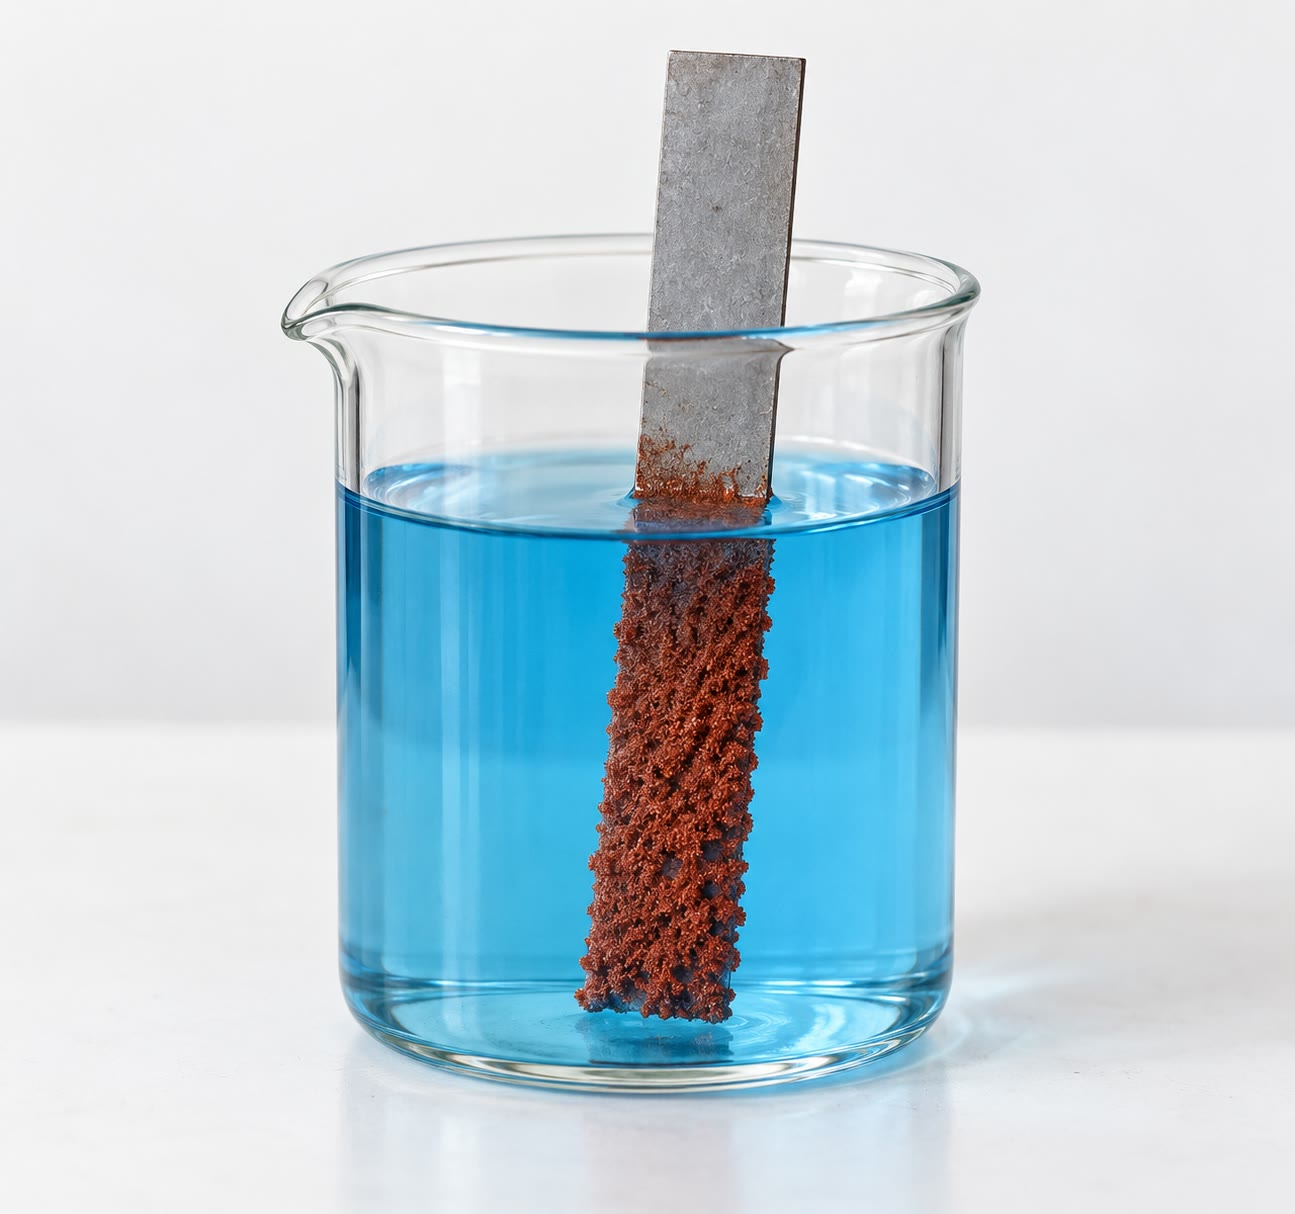
\includegraphics[width=0.55\linewidth]{images/book1/ai/g11-zinc-copper-sulfate.jpg}

{\small Una lámina de cinc en una disolución de sulfato de cobre: el
cobre se deposita sobre el cinc, y los \omterm{def:g9:ions:ion}{iones} cinc ocupan su lugar en la
disolución.}
\end{omfigure}

\section{Oxidantes y reductores}

\begin{definition}[Oxidante y reductor]\label{def:g11:redox:oxidant}
Un \emph{oxidante}\index{oxidante} es una especie capaz de ganar uno o
varios \omterm{def:g9:inside-the-atom:nucleus}{electrones}. Un \emph{reductor}\index{reductor} es una especie
capaz de ceder uno o varios \omterm{def:g9:inside-the-atom:nucleus}{electrones}.
\end{definition}

\begin{definition}[Oxidación y reducción]\label{def:g11:redox:oxidation}
Una \emph{oxidación}\index{oxidacion@oxidación} es una pérdida de \omterm{def:g9:inside-the-atom:nucleus}{electrones}; una
\emph{reducción}\index{reduccion@reducción} es una ganancia de \omterm{def:g9:inside-the-atom:nucleus}{electrones}. Un
\omterm{def:g11:redox:oxidant}{reductor} se oxida; un \omterm{def:g11:redox:oxidant}{oxidante} se reduce.
\end{definition}

\begin{remark}[Una forma de recordarlo]\label{rem:g11:redox:remember}
En una \emph{\omterm{def:g11:redox:oxidation}{reducción}} se reduce la carga de la especie: \ce{Cu^{2+}},
al ganar dos \omterm{def:g9:inside-the-atom:nucleus}{electrones}, se convierte en \ce{Cu}, carga $+2 \to 0$. En
una \omterm{def:g11:redox:oxidation}{oxidación} la carga sube: \ce{Zn -> Zn^{2+} + 2e-}, $0 \to +2$.
\end{remark}

\begin{definition}[Par redox y semiecuación]\label{def:g11:redox:couple}
Un \omterm{def:g11:redox:oxidant}{oxidante} y el \omterm{def:g11:redox:oxidant}{reductor} en que se convierte al ganar \omterm{def:g9:inside-the-atom:nucleus}{electrones}
forman un \emph{par redox}\index{par redox}, que se escribe Ox/Red con el
\omterm{def:g11:redox:oxidant}{oxidante} primero: \ce{Cu^{2+}}/\ce{Cu}, \ce{Zn^{2+}}/\ce{Zn}. El
intercambio de \omterm{def:g9:inside-the-atom:nucleus}{electrones} dentro de un par se describe con su
\emph{semiecuación}\index{semiecuacion@semiecuación},
\[
  \text{Ox} + n\,\ce{e-} \ce{<=>} \text{Red}, % ce-unbalanced-ok (generic form)
\]
ajustada en \omterm{def:g7:atoms-and-molecules:atom}{átomos} y en carga, por ejemplo
$\ce{Cu^{2+}(aq) + 2e- <=> Cu(s)}$. La doble flecha indica que el
intercambio puede ir en los dos sentidos.
\end{definition}

\begin{example}[Los metales y sus iones]\label{ex:g11:redox:metals}
Todo \omterm{def:g9:periodic-table-first-look:metal}{metal} forma un par con su \omterm{def:g9:ions:ion}{ion}:
\begin{center}
\begin{tabular}{ll}
\hline
par & \omterm{def:g11:redox:couple}{semiecuación} \\
\hline
\ce{Ag+}/\ce{Ag} & \ce{Ag+ + e- <=> Ag} \\
\ce{Cu^{2+}}/\ce{Cu} & \ce{Cu^{2+} + 2e- <=> Cu} \\
\ce{Fe^{2+}}/\ce{Fe} & \ce{Fe^{2+} + 2e- <=> Fe} \\
\ce{Zn^{2+}}/\ce{Zn} & \ce{Zn^{2+} + 2e- <=> Zn} \\
\ce{Al^{3+}}/\ce{Al} & \ce{Al^{3+} + 3e- <=> Al} \\
\hline
\end{tabular}
\end{center}
Los \omterm{def:g9:ions:ion}{iones} también pueden formar pares: \ce{Fe^{3+} + e- <=> Fe^{2+}}
para el par \ce{Fe^{3+}}/\ce{Fe^{2+}}, y \ce{I2 + 2e- <=> 2I-} para
\ce{I2}/\ce{I-}. Y también el hidrógeno: \ce{2H+ + 2e- <=> H2} para
\ce{H+}/\ce{H2}.
\end{example}

\begin{remark}[Una especie, dos papeles]\label{rem:g11:redox:amphoteric}
Una especie puede ser el \omterm{def:g11:redox:oxidant}{reductor} de un par y el \omterm{def:g11:redox:oxidant}{oxidante} de otro. El
\omterm{def:g9:ions:ion}{ion} \ce{Fe^{2+}} es el \omterm{def:g11:redox:oxidant}{oxidante} de \ce{Fe^{2+}}/\ce{Fe} y el \omterm{def:g11:redox:oxidant}{reductor} de
\ce{Fe^{3+}}/\ce{Fe^{2+}}. El papel que desempeña depende de su
compañero en la reacción.
\end{remark}

\section{Las reacciones redox}

\begin{definition}[Reacción redox]\label{def:g11:redox:reaction}
Una \emph{reacción redox}\index{reaccion redox@reacción redox} es una transferencia de
\omterm{def:g9:inside-the-atom:nucleus}{electrones} del \omterm{def:g11:redox:oxidant}{reductor} de un par al \omterm{def:g11:redox:oxidant}{oxidante} de otro. El \omterm{def:g11:redox:oxidant}{reductor} se
oxida y el \omterm{def:g11:redox:oxidant}{oxidante} se reduce, al mismo tiempo.
\end{definition}

\begin{proposition}[No hay electrones libres]\label{prop:g11:redox:no-free-electrons}
Los \omterm{def:g9:inside-the-atom:nucleus}{electrones} no existen libres en una disolución: cada \omterm{def:g9:inside-the-atom:nucleus}{electrón} que
cede el \omterm{def:g11:redox:oxidant}{reductor} lo toma el \omterm{def:g11:redox:oxidant}{oxidante}. La ecuación de una \omterm{def:g11:redox:reaction}{reacción redox}
se obtiene, por tanto, sumando las dos \omterm{def:g11:redox:couple}{semiecuaciones}, cada una
multiplicada por el número que iguala los \omterm{def:g9:inside-the-atom:nucleus}{electrones} cedidos y los
\omterm{def:g9:inside-the-atom:nucleus}{electrones} tomados; los \omterm{def:g9:inside-the-atom:nucleus}{electrones} se anulan entonces y no aparecen en
la ecuación.
\end{proposition}

\begin{example}[El cinc y los iones cobre]\label{ex:g11:redox:zinc-copper}
En la escena del principio, el cinc se oxida y los \omterm{def:g9:ions:ion}{iones} cobre se
reducen:
\[
\begin{array}{l@{\qquad}l}
  \ce{Zn(s) -> Zn^{2+}(aq) + 2e-} & \text{(oxidación)}\\
  \ce{Cu^{2+}(aq) + 2e- -> Cu(s)} & \text{(reducción)}\\
  \hline
  \ce{Zn(s) + Cu^{2+}(aq) -> Zn^{2+}(aq) + Cu(s)} &
\end{array}
\]
Dos \omterm{def:g9:inside-the-atom:nucleus}{electrones} pasan de cada \omterm{def:g7:atoms-and-molecules:atom}{átomo} de cinc a un \omterm{def:g9:ions:ion}{ion} cobre. El color azul
de la disolución es el color de los \omterm{def:g9:ions:ion}{iones} \ce{Cu^{2+}}; se atenúa a
medida que se consumen, mientras los \omterm{def:g9:ions:ion}{iones} \ce{Zn^{2+}}, incoloros,
ocupan su lugar.
\end{example}

\begin{omfigure}
\begin{tikzpicture}[font=\small, >=Stealth,
    ion/.style={circle, draw=black!70, minimum size=10mm, inner sep=0pt}]
  % the zinc strip and the solution
  \fill[black!18] (0,0) rectangle (1.6,4);
  \draw[black!60] (1.6,0) -- (1.6,4);
  \node[anchor=south] at (0.8,0.08) {cinc};
  \fill[omWater!60] (1.6,0) rectangle (9.0,4);
  \node[anchor=north east] at (8.95,3.95) {disolución};
  % a zinc atom leaves as an ion
  \node[ion, fill=black!30] (zn) at (1.15,3.0) {\ce{Zn}};
  \node[ion, fill=white] (znion) at (5.0,3.0) {\ce{Zn^{2+}}};
  \draw[->, thick, omProp] (zn.east) -- (znion.west)
    node[midway, above] {oxidación};
  % the electrons travel through the metal
  \draw[->, thick, omDef, dashed] (0.75,2.45) -- (0.75,1.55)
    node[midway, right] {2\,\ce{e-}};
  % a copper ion is reduced on the surface
  \node[ion, fill=omDef!35] (cuion) at (5.0,1.0) {\ce{Cu^{2+}}};
  \node[ion, fill=orange!55!brown] (cu) at (2.12,1.0) {\ce{Cu}};
  \draw[->, thick, omProp] (cuion.west) -- (cu.east)
    node[midway, above] {reducción};
  \node[anchor=west, align=left] at (6.1,2.0) {cada átomo de cinc cede\\ dos electrones a un\\ ion cobre};
\end{tikzpicture}

{\small En la superficie del cinc. Un \omterm{def:g7:atoms-and-molecules:atom}{átomo} de cinc pierde dos \omterm{def:g9:inside-the-atom:nucleus}{electrones}
y se va como \omterm{def:g9:ions:ion}{ion} \ce{Zn^{2+}}; los dos \omterm{def:g9:inside-the-atom:nucleus}{electrones} viajan por el \omterm{def:g9:periodic-table-first-look:metal}{metal}
hasta un \omterm{def:g9:ions:ion}{ion} \ce{Cu^{2+}} que toca la superficie, que se convierte en un
\omterm{def:g7:atoms-and-molecules:atom}{átomo} de cobre y se queda sobre la lámina.}
\end{omfigure}

\begin{omfigure}
\begin{tikzpicture}[font=\small]
  \pic at (0,0) {beaker={0.75}{omDef!45}};
  \fill[black!35] (-0.15,0.25) rectangle (0.15,2.5);
  \draw[black!65] (-0.15,0.25) rectangle (0.15,2.5);
  \node[anchor=north, align=center] at (0,-0.15) {al principio:\\ disolución azul de \ce{Cu^{2+}}};
  \draw[->, thick, omProp] (1.3,1) -- (3.2,1) node[midway, above] {una hora};
  \pic at (4.5,0) {beaker={0.75}{omDef!12}};
  \fill[black!35] (4.35,0.25) rectangle (4.65,2.5);
  \fill[orange!55!brown] (4.3,0.25) rectangle (4.7,1.5);
  \draw[black!65] (4.35,0.25) rectangle (4.65,2.5);
  \node[anchor=north, align=center] at (4.5,-0.15) {después: disolución más clara,\\ cobre sobre el cinc};
\end{tikzpicture}

{\small Lo que se ve: el depósito de cobre en la parte sumergida de la
lámina, y la atenuación del color azul de los \omterm{def:g9:ions:ion}{iones} \ce{Cu^{2+}}.}
\end{omfigure}

\begin{example}[Los metales en ácido, otra vez]\label{ex:g11:redox:acid}
Cuando el hierro se \omterm{def:g2:mixing-and-dissolving:dissolve}{disuelve} en ácido clorhídrico, el hierro se oxida y
los \omterm{def:g9:ions:ion}{iones} \ce{H+} se reducen a hidrógeno:
\[
  \ce{Fe(s) + 2H+(aq) -> Fe^{2+}(aq) + H2(g)}.
\]
Los pares son \ce{Fe^{2+}}/\ce{Fe} y \ce{H+}/\ce{H2}; los \omterm{def:g9:ions:ion}{iones} cloruro
no intervienen.
\end{example}

\begin{inthelab}[El árbol de plata]
Se cuelga una espiral de hilo de cobre limpio en un vaso de
precipitados con una disolución diluida de nitrato de plata,
\ce{Ag+(aq) + NO3^-(aq)}. En menos de una hora crecen a lo largo del
hilo unas agujas ramificadas de plata brillante, y la disolución
incolora se vuelve azul pálido:
\ce{Cu(s) + 2Ag+(aq) -> Cu^{2+}(aq) + 2Ag(s)}. El experimento lo hace el
profesor, con guantes y gafas, y después la disolución se recoge como
residuo peligroso.
\end{inthelab}

\begin{safety}{\ghs[0.82cm]{GHS03}\ghs[0.82cm]{GHS05}\ghs[0.82cm]{GHS08}\ghs[0.82cm]{GHS09}}
% ledger: ghs:AgNO3
Nitrato de plata: un comburente que puede avivar un incendio (GHS03);
corrosivo para la piel y los ojos, y mancha la piel de negro (GHS05);
peligroso para la salud (GHS08); muy tóxico para los organismos
acuáticos, así que nunca se tira por el fregadero (GHS09).
\end{safety}

\begin{omfigure}
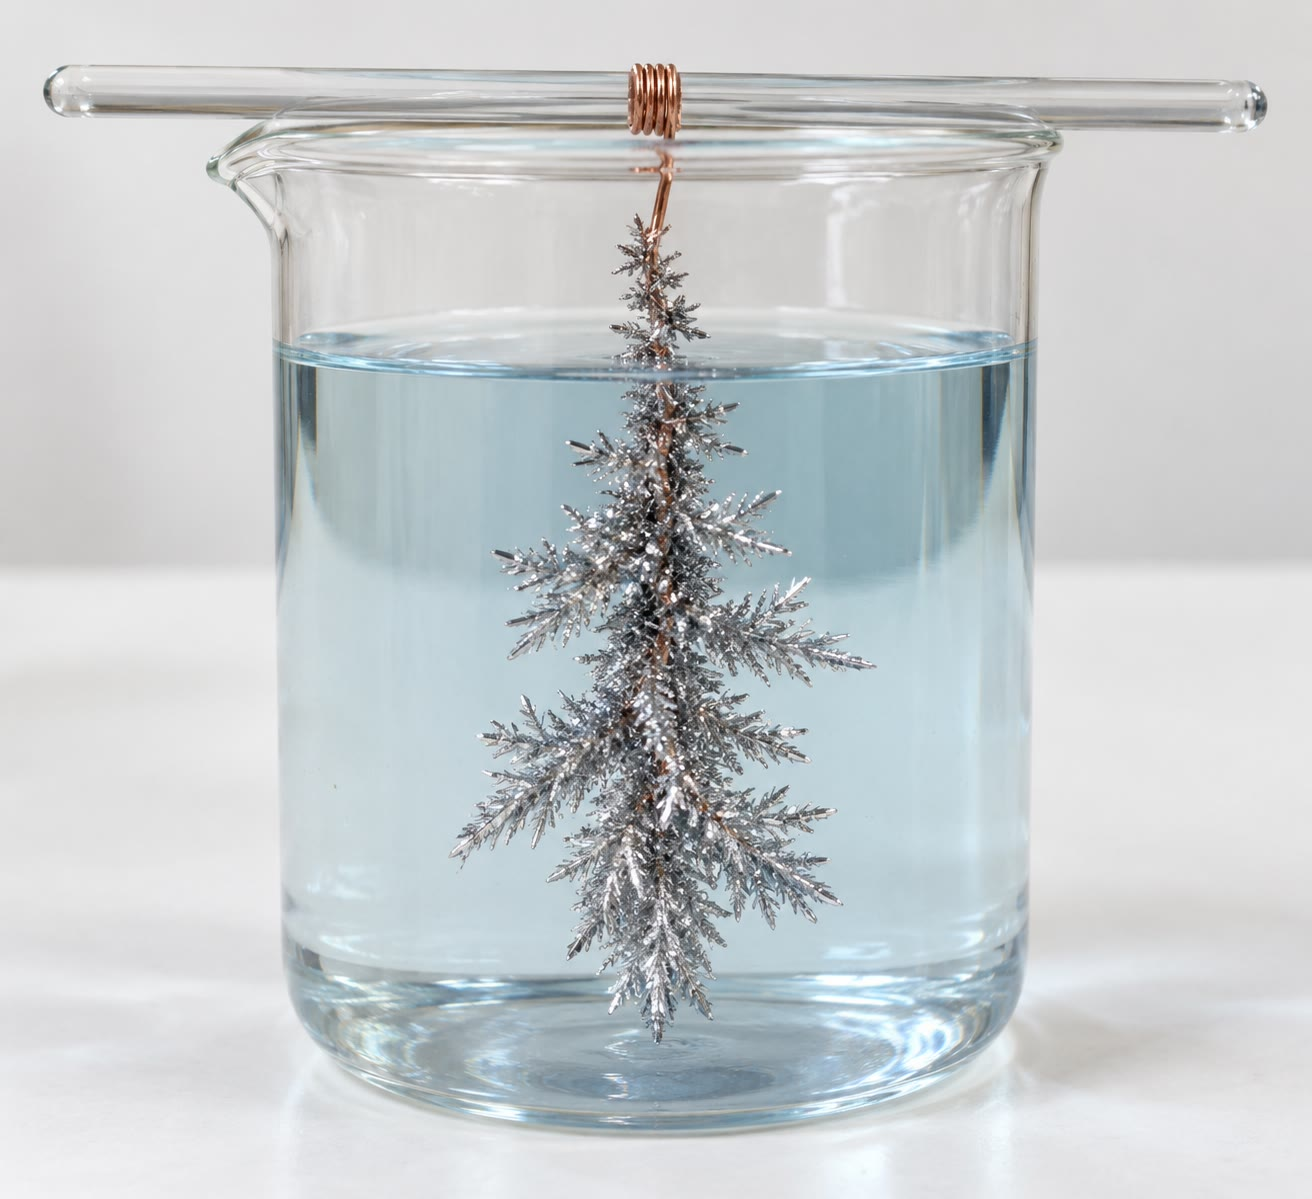
\includegraphics[width=0.5\linewidth]{images/book1/ai/g11-silver-tree.jpg}

{\small Cristales de plata que crecen sobre un hilo de cobre en una
disolución de nitrato de plata.}
\end{omfigure}

\section{Ajustar semiecuaciones}

Muchos pares importantes contienen oxígeno y se escriben para
\omterm{def:g9:acids-bases-ph:acidic}{disoluciones ácidas}, donde hay \omterm{def:g9:ions:ion}{iones} \ce{H+}. Sus \omterm{def:g11:redox:couple}{semiecuaciones}
necesitan \omterm{def:g7:atoms-and-molecules:molecule}{moléculas} de agua e \omterm{def:g9:ions:ion}{iones} \ce{H+} para ajustarse.

\begin{method}[Ajustar una semiecuación en disolución ácida]\label{met:g11:redox:balance}
Para escribir la \omterm{def:g11:redox:couple}{semiecuación} de un par Ox/Red en \omterm{def:g9:acids-bases-ph:acidic}{disolución ácida}:
\begin{enumerate}
  \item escribir Ox a la izquierda y Red a la derecha, y ajustar el
        \omterm{def:g7:atoms-and-molecules:atom}{átomo} que no es ni O ni H;
  \item ajustar los \omterm{def:g7:atoms-and-molecules:atom}{átomos} de oxígeno con \omterm{def:g7:atoms-and-molecules:molecule}{moléculas} de agua \ce{H2O};
  \item ajustar los \omterm{def:g7:atoms-and-molecules:atom}{átomos} de hidrógeno con \omterm{def:g9:ions:ion}{iones} \ce{H+};
  \item ajustar la carga con \omterm{def:g9:inside-the-atom:nucleus}{electrones} \ce{e-}, a la izquierda;
  \item comprobar: el mismo número de cada \omterm{def:g7:atoms-and-molecules:atom}{átomo} y la misma carga total
        en los dos miembros.
\end{enumerate}
\end{method}

\begin{example}[El ion permanganato]\label{ex:g11:redox:permanganate}
Para el par \ce{MnO4^-}/\ce{Mn^{2+}} (de violeta intenso a casi
incoloro): el manganeso está ajustado; los cuatro O de la izquierda dan
$\ce{4H2O}$ a la derecha; sus ocho H dan $\ce{8H+}$ a la izquierda; la
carga de la izquierda es $-1 + 8 = +7$, y la de la derecha, $+2$, así
que se añaden cinco \omterm{def:g9:inside-the-atom:nucleus}{electrones} a la izquierda:
\[
  \ce{MnO4^-(aq) + 8H+(aq) + 5e- <=> Mn^{2+}(aq) + 4H2O(l)}.
\]
\end{example}

\begin{example}[El ion dicromato]\label{ex:g11:redox:dichromate}
Para \ce{Cr2O7^{2-}}/\ce{Cr^{3+}} (de naranja a verde): dos \omterm{def:g7:atoms-and-molecules:atom}{átomos} de
cromo a la derecha; siete O dan \ce{7H2O}; catorce H dan \ce{14H+};
carga $-2 + 14 = +12$ a la izquierda frente a $2 \times 3 = +6$ a la
derecha, así que seis \omterm{def:g9:inside-the-atom:nucleus}{electrones}:
\[
  \ce{Cr2O7^{2-}(aq) + 14H+(aq) + 6e- <=> 2Cr^{3+}(aq) + 7H2O(l)}.
\]
\end{example}

\begin{method}[Escribir una ecuación redox]\label{met:g11:redox:combine}
Para escribir la ecuación de la reacción entre el \omterm{def:g11:redox:oxidant}{oxidante} Ox$_1$ de un
par y el \omterm{def:g11:redox:oxidant}{reductor} Red$_2$ de otro:
\begin{enumerate}
  \item escribir las dos \omterm{def:g11:redox:couple}{semiecuaciones}, la primera en el sentido de la
        \omterm{def:g11:redox:oxidation}{reducción} (Ox$_1 \to$ Red$_1$), y la segunda en el sentido de la
        \omterm{def:g11:redox:oxidation}{oxidación} (Red$_2 \to$ Ox$_2$);
  \item multiplicarlas por los números más pequeños que igualan los
        \omterm{def:g9:inside-the-atom:nucleus}{electrones};
  \item sumarlas; los \omterm{def:g9:inside-the-atom:nucleus}{electrones} se anulan, y también pueden anularse
        algunos \ce{H+} y \ce{H2O} que aparecen en los dos miembros;
  \item comprobar una vez más los \omterm{def:g7:atoms-and-molecules:atom}{átomos} y la carga.
\end{enumerate}
\end{method}

\begin{example}[El permanganato y el hierro(II)]\label{ex:g11:redox:mno4-fe}
El \omterm{def:g9:ions:ion}{ion} permanganato oxida los \omterm{def:g9:ions:ion}{iones} \ce{Fe^{2+}} a \ce{Fe^{3+}}:
\[
\begin{array}{l@{\qquad}l}
  \ce{MnO4^- + 8H+ + 5e- -> Mn^{2+} + 4H2O} & \times 1\\
  \ce{Fe^{2+} -> Fe^{3+} + e-} & \times 5\\
  \hline
  \ce{MnO4^- + 8H+ + 5Fe^{2+} -> Mn^{2+} + 5Fe^{3+} + 4H2O} &
\end{array}
\]
Carga a la izquierda: $-1 + 8 + 10 = +17$; a la derecha: $2 + 15 = +17$.
Esta reacción se usa en el capítulo siguiente para medir una cantidad
de hierro(II).
\end{example}

\section{Oxidantes y reductores a nuestro alrededor}

\begin{proposition}[Algunos oxidantes y reductores corrientes]\label{prop:g11:redox:common}
Las especies siguientes aparecen una y otra vez en el laboratorio y en
la vida diaria:
\begin{center}
\small
\begin{tabular}{lll}
\hline
especie & papel & \omterm{def:g11:redox:couple}{semiecuación} de su par \\
\hline
dioxígeno \ce{O2} & \omterm{def:g11:redox:oxidant}{oxidante} & \ce{O2 + 4H+ + 4e- <=> 2H2O} \\
dicloro \ce{Cl2} & \omterm{def:g11:redox:oxidant}{oxidante} & \ce{Cl2 + 2e- <=> 2Cl-} \\
hipoclorito \ce{ClO-} (lejía) & \omterm{def:g11:redox:oxidant}{oxidante} & \ce{2ClO- + 4H+ + 2e- <=> Cl2 + 2H2O} \\
peróxido de hidrógeno \ce{H2O2} & \omterm{def:g11:redox:oxidant}{oxidante} & \ce{H2O2 + 2H+ + 2e- <=> 2H2O} \\
permanganato \ce{MnO4^-} & \omterm{def:g11:redox:oxidant}{oxidante} & \ce{MnO4^- + 8H+ + 5e- <=> Mn^{2+} + 4H2O} \\
\omterm{def:g9:periodic-table-first-look:metal}{metales} \ce{M} (\ce{Fe}, \ce{Zn}, \ce{Al}\dots) & \omterm{def:g11:redox:oxidant}{reductores} & \ce{M^{n+} + $n$ e- <=> M} % ce-unbalanced-ok (generic)
\\
yoduro \ce{I-} & \omterm{def:g11:redox:oxidant}{reductor} & \ce{I2 + 2e- <=> 2I-} \\
tiosulfato \ce{S2O3^{2-}} & \omterm{def:g11:redox:oxidant}{reductor} & \ce{S4O6^{2-} + 2e- <=> 2S2O3^{2-}} \\
ácido ascórbico \ce{C6H8O6} (vitamina C) & \omterm{def:g11:redox:oxidant}{reductor} & \ce{C6H6O6 + 2H+ + 2e- <=> C6H8O6} \\
\hline
\end{tabular}
\end{center}
\end{proposition}

\begin{example}[El cobre se vuelve verde]\label{ex:g11:redox:patina}
Los tejados y las estatuas de cobre, al \omterm{def:g4:air-a-mixture-of-gases:air}{aire} libre durante décadas, se
van volviendo de un verde pálido. El oxígeno del \omterm{def:g4:air-a-mixture-of-gases:air}{aire} oxida el cobre a
\omterm{def:g9:ions:ion}{iones} \ce{Cu^{2+}}, que, con el agua y el dióxido de carbono, forman una
fina costra verde, la pátina. A diferencia de la \omterm{def:g9:metals-acids-corrosion:corrosion}{herrumbre} del hierro,
la pátina se adhiere al \omterm{def:g9:periodic-table-first-look:metal}{metal} y lo protege de nuevos ataques.
\end{example}

\begin{omfigure}

\includegraphics[width=0.48\linewidth]{images/book1/ai/g11-green-roof.jpg}

{\small Un tejado de cobre después de décadas al \omterm{def:g4:air-a-mixture-of-gases:air}{aire}: el cobre oxidado
forma una pátina verde.}
\end{omfigure}

\begin{remark}[Los antioxidantes]\label{rem:g11:redox:antioxidant}
Un ``antioxidante'' añadido a un alimento es un \omterm{def:g11:redox:oxidant}{reductor} que el oxígeno
del \omterm{def:g4:air-a-mixture-of-gases:air}{aire} oxida antes que al alimento. La vitamina C (ácido ascórbico) es
el más corriente: una manzana cortada rociada con zumo de limón se pone
marrón mucho más despacio, porque la vitamina C del limón se oxida
primero.
\end{remark}

\section{Ejercicios}

\begin{exercise}[$\star$]\label{exo:g11:redox:1}
Define un \omterm{def:g11:redox:oxidant}{oxidante}, un \omterm{def:g11:redox:oxidant}{reductor}, una \omterm{def:g11:redox:oxidation}{oxidación} y una \omterm{def:g11:redox:oxidation}{reducción}.
\end{exercise}

\begin{exercise}[$\star$]\label{exo:g11:redox:2}
Para cada pareja, escribe el \omterm{def:g11:redox:couple}{par redox} en la forma Ox/Red: \ce{Fe} y
\ce{Fe^{2+}}; \ce{Ag} y \ce{Ag+}; \ce{I-} y \ce{I2}; \ce{Fe^{2+}} y
\ce{Fe^{3+}}.
\end{exercise}

\begin{exercise}[$\star$]\label{exo:g11:redox:3}
Escribe las \omterm{def:g11:redox:couple}{semiecuaciones} de los pares \ce{Ag+}/\ce{Ag},
\ce{Al^{3+}}/\ce{Al}, \ce{Fe^{3+}}/\ce{Fe^{2+}} y \ce{Cl2}/\ce{Cl-}.
\end{exercise}

\begin{exercise}[$\star$]\label{exo:g11:redox:4}
¿La transformación \ce{Fe -> Fe^{2+} + 2e-} es una \omterm{def:g11:redox:oxidation}{oxidación} o una
\omterm{def:g11:redox:oxidation}{reducción}? ¿Actúa el hierro como \omterm{def:g11:redox:oxidant}{oxidante} o como \omterm{def:g11:redox:oxidant}{reductor}?
\end{exercise}

\begin{exercise}[$\star$]\label{exo:g11:redox:5}
En la reacción \ce{Zn + Cu^{2+} -> Zn^{2+} + Cu}, nombra la especie
oxidada, la especie reducida, el \omterm{def:g11:redox:oxidant}{oxidante} y el \omterm{def:g11:redox:oxidant}{reductor}, y da el número
de \omterm{def:g9:inside-the-atom:nucleus}{electrones} transferidos por cada \omterm{def:g7:atoms-and-molecules:atom}{átomo} de cinc.
\end{exercise}

\begin{exercise}[$\star\star$]\label{exo:g11:redox:6}
Ajusta, en \omterm{def:g9:acids-bases-ph:acidic}{disolución ácida}, la \omterm{def:g11:redox:couple}{semiecuación} del par
\ce{H2O2}/\ce{H2O}, siguiendo paso a paso el
\cref{met:g11:redox:balance}.
\end{exercise}

\begin{exercise}[$\star\star$]\label{exo:g11:redox:7}
Escribe la ecuación de la reacción entre el yodo \ce{I2} y el \omterm{def:g9:ions:ion}{ion}
tiosulfato \ce{S2O3^{2-}}, que da \omterm{def:g9:ions:ion}{iones} yoduro e \omterm{def:g9:ions:ion}{iones} tetrationato
\ce{S4O6^{2-}}.
\end{exercise}

\begin{exercise}[$\star\star$]\label{exo:g11:redox:8}
Escribe la ecuación de la reacción del árbol de plata a partir de sus
dos \omterm{def:g11:redox:couple}{semiecuaciones}, y explica por qué la disolución se vuelve azul.
\end{exercise}

\begin{exercise}[$\star\star$]\label{exo:g11:redox:9}
La vitamina C, \ce{C6H8O6}, reacciona con el yodo \ce{I2}. Escribe la
ecuación de la reacción, y di qué especie es el \omterm{def:g11:redox:oxidant}{reductor}.
\end{exercise}

\begin{exercise}[$\star\star$]\label{exo:g11:redox:10}
El aluminio reacciona con los \omterm{def:g9:ions:ion}{iones} cobre(II). Escribe la ecuación, y
explica por qué hay que multiplicar las \omterm{def:g11:redox:couple}{semiecuaciones} por 2 y por 3.
\end{exercise}

\begin{exercise}[$\star\star$]\label{exo:g11:redox:11}
El peróxido de hidrógeno oxida los \omterm{def:g9:ions:ion}{iones} hierro(II) a \omterm{def:g9:ions:ion}{iones} hierro(III)
en \omterm{def:g9:acids-bases-ph:acidic}{disolución ácida}. Escribe la ecuación.
\end{exercise}

\begin{exercise}[$\star\star\star$]\label{exo:g11:redox:12}
Una lámina de cinc pierde \qty{1.30}{g} en una disolución que contiene
un exceso de \omterm{def:g9:ions:ion}{iones} cobre(II). ¿Qué masa de cobre se deposita? Toma
$M(\ce{Zn}) = \qty{65.4}{g/mol}$ y $M(\ce{Cu}) = \qty{63.5}{g/mol}$.
\end{exercise}

\begin{exercise}[$\star\star\star$]\label{exo:g11:redox:13}
Escribe la ecuación de la \omterm{def:g11:redox:oxidation}{oxidación} de los \omterm{def:g9:ions:ion}{iones} hierro(II) por los
\omterm{def:g9:ions:ion}{iones} dicromato en \omterm{def:g9:acids-bases-ph:acidic}{disolución ácida}. ¿Qué cantidad de \ce{Fe^{2+}}
oxidan \qty{0.010}{mol} de \omterm{def:g9:ions:ion}{iones} dicromato?
\end{exercise}

\begin{exercise}[$\star\star\star$]\label{exo:g11:redox:14}
La lejía contiene \omterm{def:g9:ions:ion}{iones} hipoclorito \ce{ClO-} e \omterm{def:g9:ions:ion}{iones} cloruro \ce{Cl-}.
Con los pares \ce{ClO-}/\ce{Cl2} y \ce{Cl2}/\ce{Cl-}, escribe la
ecuación de la reacción que se produce cuando la lejía entra en contacto
con un ácido, y explica por qué las etiquetas de la lejía y de los
desincrustantes ácidos advierten de que no se deben \omterm{def:g2:mixing-and-dissolving:mix}{mezclar} nunca.
\end{exercise}

\begin{exercise}[$\star\star\star$]\label{exo:g11:redox:15}
En la figura de la superficie del cinc, los \omterm{def:g9:inside-the-atom:nucleus}{electrones} viajan por el
\omterm{def:g9:periodic-table-first-look:metal}{metal}, no por la disolución. Con la
\cref{prop:g11:redox:no-free-electrons}, explica por qué el cobre se
deposita sobre la propia lámina de cinc y no en otro lugar del vaso.
\end{exercise}

\section{Problema: El alcoholímetro}

\begin{problem}[{Problema de fin de semana --- la química de un tubo
alcoholímetro: dos pares, un cambio de color de naranja a verde, la masa
de etanol que puede detectar un tubo y la pila de combustible que lo
sustituyó}]
\label{pb:g11:redox:1}
% ledger: ghs:K2Cr2O7, breath:ratio; molar masses from tools/molar_mass.py
% (0.1-rounded weights): K2Cr2O7 294.2, C2H6O 46.0 g/mol
Los primeros controles de alcoholemia en \omterm{def:g4:air-a-mixture-of-gases:air}{aire} espirado usaban un tubo de
vidrio relleno de granos de sílice recubiertos de dicromato de potasio
naranja, \ce{K2Cr2O7}, en medio ácido. El etanol, \ce{CH3CH2OH}, del
aliento soplado a través del tubo reduce los \omterm{def:g9:ions:ion}{iones} dicromato a \omterm{def:g9:ions:ion}{iones}
\ce{Cr^{3+}} verdes y se oxida a ácido etanoico, \ce{CH3COOH}; la
longitud de la zona verde mide el etanol. Supón que un tubo contiene
\qty{2.0}{mg} de dicromato de potasio. Usa
$M(\ce{K}) = 39.1$, $M(\ce{Cr}) = 52.0$, $M(\ce{O}) = 16.0$,
$M(\ce{C}) = 12.0$, $M(\ce{H}) = \qty{1.0}{g/mol}$, $N_A =
\qty{6.02e23}{mol^{-1}}$ y $e = \qty{1.60e-19}{C}$.

\medskip
\noindent\textbf{Parte I --- Dos pares.}
\begin{enumerate}
  \item Nombra los dos \omterm{def:g11:redox:couple}{pares redox} que intervienen, con el \omterm{def:g11:redox:oxidant}{oxidante}
        primero.
  \item ¿El etanol se oxida o se reduce? ¿Es el \omterm{def:g11:redox:oxidant}{oxidante} o el \omterm{def:g11:redox:oxidant}{reductor}?
  \item Escribe la \omterm{def:g11:redox:couple}{semiecuación} del par \ce{Cr2O7^{2-}}/\ce{Cr^{3+}} en
        \omterm{def:g9:acids-bases-ph:acidic}{disolución ácida}.
  \item Escribe la \omterm{def:g11:redox:couple}{semiecuación} del par \ce{CH3COOH}/\ce{CH3CH2OH} en
        \omterm{def:g9:acids-bases-ph:acidic}{disolución ácida}.
  \item Deduce la ecuación de la reacción que tiene lugar en el tubo.
\end{enumerate}

\medskip
\noindent\textbf{Parte II --- Lo que puede medir un tubo.}
\begin{enumerate}[resume]
  \item Explica el cambio de color de los granos.
  \item Calcula la \omterm{def:g10:the-mole:molar-mass}{masa molar} del dicromato de potasio.
  \item Calcula la cantidad de \omterm{def:g9:ions:ion}{iones} dicromato del tubo.
  \item ¿Qué cantidad de etanol hace falta para que todo el tubo se
        vuelva verde?
  \item Deduce la mayor masa de etanol que puede medir un tubo.
\end{enumerate}

\medskip
\noindent\textbf{Parte III --- Del aliento a la sangre.}
Una persona sopla \qty{1.0}{L} de \omterm{def:g4:air-a-mixture-of-gases:air}{aire} espirado a través del tubo; la
zona verde crece en proporción a la masa de etanol que llega a ella.
\begin{enumerate}[resume]
  \item El aliento contiene \qty{0.25}{mg} de etanol por litro. ¿Qué
        fracción del dicromato se gasta?
  \item El tubo mide \qty{10}{cm} de largo. ¿Qué longitud tiene la zona
        verde?
  \item Los alcoholímetros suponen que \qty{2100}{L} de \omterm{def:g4:air-a-mixture-of-gases:air}{aire} espirado
        contienen tanto etanol como \qty{1}{L} de sangre. Estima la masa
        de etanol por litro de sangre, en gramos.
  \item ¿Por qué la zona verde empieza en la entrada del tubo y crece
        hacia la salida, en lugar de volverse todo el tubo ligeramente
        verde?
  \item ¿Por qué un tubo solo se puede usar una vez?
\end{enumerate}

\medskip
\noindent\textbf{Parte IV --- La pila de \omterm{def:g4:what-a-fire-needs:fuel}{combustible}.}
El dicromato de potasio lleva los pictogramas
\ghs[0.6cm]{GHS03}\,\ghs[0.6cm]{GHS05}\,\ghs[0.6cm]{GHS06}\,\ghs[0.6cm]{GHS07}\,\ghs[0.6cm]{GHS08}\,\ghs[0.6cm]{GHS09}.
Los aparatos modernos usan en su lugar una pila de \omterm{def:g4:what-a-fire-needs:fuel}{combustible}, en la
que el etanol del aliento se oxida con dioxígeno sobre un electrodo, y
los \omterm{def:g9:inside-the-atom:nucleus}{electrones} liberados circulan por un cable.
\begin{enumerate}[resume]
  \item Da dos razones, leídas en los pictogramas, por las que se
        abandonaron los tubos de dicromato.
  \item Escribe la ecuación de la \omterm{def:g11:redox:oxidation}{oxidación} del etanol por el
        dioxígeno, usando el par \ce{O2}/\ce{H2O}.
  \item ¿Cuántos \omterm{def:g9:inside-the-atom:nucleus}{electrones} cede una \omterm{def:g7:atoms-and-molecules:molecule}{molécula} de etanol cuando se oxida
        a ácido etanoico?
  \item Para \qty{0.25}{mg} de etanol, calcula la cantidad de etanol y,
        después, el número de \omterm{def:g9:inside-the-atom:nucleus}{electrones} liberados.
  \item Deduce la carga eléctrica que circula por la pila de
        \omterm{def:g4:what-a-fire-needs:fuel}{combustible}. ¿Por qué esta carga es una buena medida del etanol
        del aliento?
\end{enumerate}
\end{problem}
